\documentclass{article}

\textwidth=6.5in
\textheight=8.5in
\voffset=-54pt
\oddsidemargin=0in
\evensidemargin=0in
\setlength{\parskip}{8pt}
\setlength{\parindent}{0pt}

\usepackage{amsmath, amssymb}
\usepackage{ifthen}

\usepackage[inline]{enumitem}
\setlist{topsep=0pt, parsep=8pt}

\usepackage[rgb,table]{xcolor}\convertcolorsUfalse
\usepackage{graphicx}

% change hyperref options
\PassOptionsToPackage{hyphens}{url}
\usepackage[bookmarks,colorlinks,linkcolor=black,citecolor=blue,pdfstartview=FitH,urlcolor=blue]{hyperref}
\hypersetup{pdfpagemode=UseNone}
\usepackage{bookmark}

\usepackage{graphicx}
\usepackage{multicol}
\usepackage{framed}
\usepackage{array}

\usepackage{icomma}

\usepackage{soul}

\usepackage{tikz}
\usetikzlibrary{
  matrix,%
  % enables the snake paths
  decorations.pathmorphing,%
  % enables bigger arrows
  decorations.markings,%
  decorations.pathreplacing,%
  decorations.text,%
  calc,%
  patterns,%
  shapes.geometric,%
  arrows,
  decorations.shapes,
  positioning,
  plotmarks,
  intersections
}
\tikzset{>=latex} % sets default arrow type in tikz
\tikzset{font=\normalsize}
\tikzset{mark size=1.5pt, mark options=thin}
\tikzset{pin distance=4pt,
  every pin edge/.style={<-, thin, shorten <= -2pt}}

\interfootnotelinepenalty=10000
\renewcommand{\thefootnote}{(\arabic{footnote})}

\usepackage{multirow, bigdelim}

% change to \usepackage[sols]{handout} to see solutions
\usepackage[sols,workshop,grading]{handout}
\renewcommand{\workshopnote}{CA Notes.}    

\newcommand\iscurrentenumi[1]{%
  \ifthenelse{\equal{#1}{\theenumi}}{}{#1}}
\setenumerate[1]{ref=\#\arabic*}
\setenumerate[2]{ref=\protect\iscurrentenumi{\theenumi}(\alph*)}
\newcommand\enumiiprefix[2]{%
  \ifthenelse{{\equal{#1}{\theenumi}}\AND{\equal{#2}{(\alph{enumii})}}}{}{}%
  \ifthenelse{{\equal{#1}{\theenumi}}\AND{\NOT{\equal{#2}{(\alph{enumii})}}}}{#2}{}%
  \ifthenelse{\equal{#1}{\theenumi}}{}{#1#2}%
}
\setenumerate[3]{ref=\protect\enumiiprefix{\theenumi}{(\alph{enumii})}\roman*}

\definecolor{purple}{rgb}{0.5,0,1.0}
\definecolor{hotpink}{rgb}{1, 0, 0.5}
\definecolor{skyblue}{rgb}{0, 0.5, 1}

\newcommand{\goal}[1]{\textbf{\textcolor{skyblue}{#1}}}
\newcommand{\indvar}[1]{\textbf{\textcolor{hotpink}{#1}}}

\newcommand{\doedfinity}[2][\newpage]{
  \begin{problem}[#1]
    Do the Edfinity assignment ``Problem Set #2''.

    We encourage you to write down any scratch work here, as well as
    things you want your future self to remember. Nothing you write
    here will be graded; it's just for you!
  \end{problem}
}

\newcommand{\psreflection}[2][]{

  \ifthenelse{\not\equal{#1}{nocite}}{
    \begin{enumerate}[resume]
    \item
      \begin{problem}[1in]
        Please cite any help you got on this problem set:
        \begin{itemize}[nosep]
        \item If you worked with other students, please list their names here.
        \item If you used resources other than those on our Canvas site, please list them here.
        \end{itemize}
      \end{problem}

    \end{enumerate}
  }

  \probonly{%
    #2

    \newpage

    \emph{Reflection space.} It's a good habit to take a few minutes at the end of each pset to reflect on what you learned and jot down notes to your future self. Here are a few reflection questions to get you started. Nothing you write here will be graded; it's just for you!
    \begin{itemize}
    \item Take a few minutes to look back at the problems. How could you explain to someone else how to do each problem? What was your strategy, and how did you know to use that strategy? If there are problems where you don't feel able to answer this, write down which ones they are. Come back to them in a few days when we post the homework solutions!

      \vspace{1.5in}

    \item Take a look back at the learning objectives on today's worksheet; how are you feeling about each one? If there are ones you know you need more practice with, write those down here.

      \vspace{1.5in}

    \item What did you find most challenging about this material? Do you have any lingering questions about it? If so, write them down here so you don't forget them. At some point, stop by office hours or MQC to ask!

      \vfill
    \end{itemize}      
  }
}

\usepackage{fancyhdr}
\lhead{\textcolor{white}{This content is protected and may not be shared, uploaded, or distributed.}}
\rhead{}
\rfoot{\vspace*{\fill}\footnotesize\textcopyright{} \emph{Harvard Math Ma}}
\renewcommand{\headrulewidth}{0pt}
\pagestyle{fancy}
\begin{document}

\begin{center}
  \large\textsc{Problem Set 6 - Function Composition, Modeling with Functions}
\end{center}

\begin{enumerate}
\item  \note{
    \begin{itemize}[nosep]
    \item Algebra: solving equations with fractions / square roots
    \item Composing functions given by formulas
    \item Calculating values of function composition given graphs / tables
    \item Interpreting a composition in context
    \item A photo is printed on a sheet of paper whose width and height are given. Once the photo is printed, there are $m$ inches of blank space on each side of the photo. Find the area and perimeter of the printed photo. 
    \end{itemize}
}

  \doedfinity{6}

\end{enumerate}
\begin{workshop}
  One reason we ask students to follow the steps below is that
  modeling is often just the first step to solving a more complicated
  problem (for example, later in Math M, we'll look at optimization
  and related rates, which both start with modeling). Students tend to
  become overwhelmed by the complexity if they don't approach such
  problems methodically. So, really encourage them now to develop
  these habits that will help them later!  
\end{workshop}

For full credit on modeling problems like \ref{modeling-fence-3-sides} - \ref{gottlieb-1.3.30}, please do the following in each problem:
{
  \begin{itemize}[nosep]
  \item State the goal and the information you're given.
  \item Draw a picture, explicitly labeling both variables and constants.
  \item Clearly communicate your thought process, one step at a time. 
  \end{itemize}
}

\begin{problemonly}
  \emph{Being able to model the world mathematically is often the first step in applying calculus to solve real world problems. Since this type of modeling is such an important skill, you can expect to practice more modeling on upcoming psets.}
\end{problemonly}

\begin{enumerate}[resume]
\item \label{modeling-fence-3-sides} % based on 1.3.44

  A gardener wants to put a tomato garden next to her house. She needs to fence the garden in to prevent rabbits from eating her tomatoes. One side of the garden will be against the house, so that side doesn't need any fencing. The gardener plans to use 40 feet of fence for her garden.

  \begin{enumerate}
  \item
    \begin{grading}
      5.5 points:
      \begin{itemize}[nosep]
      \item 1 for drawing a picture
      \item 0.5 for labeling the sides in the picture
      \item 1 point for stating the goal
      \item 1 point for writing down correct equation about perimeter
      \item 1 point for solving their perimeter equation for the length of the sides perpendicular to the house
      \item 1 point for plugging that into the area
      \end{itemize}
    \end{grading}

    \begin{workshop}
      This problem is very similar to {{\#3}} on \href{https://people.math.harvard.edu/~jjchen/mathma/docs/worksheets/worksheet06-sols.html}{the worksheet ``Function Composition, Modeling with Functions''}, 
      so if students have trouble, ask them to walk you through that
      problem first and to identify what's different in this problem.
    \end{workshop}

    \begin{problem}[\vfill]
      Express the area of the garden as a function of the length of
      the side that's against the house.
    \end{problem}

      \begin{solution}

        \begin{itemize}
        \item \hl{\textbf{Goal:}} Express the \goal{area} of the garden as a function of the 
        \indvar{length of the side against the house}.

          \hl{\textbf{Know:}} perimeter = 40 feet

      \item Since our goal is the \goal{area}, let's \hl{\textbf{write a formula}} for it, \hl{\textbf{defining any variables we use}} (either in words or by labeling them in a picture).

        \begin{center}
          \begin{tikzpicture}[scale = .2]
            \draw (0, 0) --  node[midway, below] {$\ell$ } (9,0) -- node[midway, right] {$w$} (9,5) -- (0,5); 
            \draw (20, 2.5) node{$\color{skyblue}{\text{area}} = A\color{black} = \ell w$};
            \draw[ultra thick, lightgray] (0,-1) -- (0, 6); 
          \end{tikzpicture}
        \end{center}

      \item Now, we need to \hl{\textbf{relate the variables we've used}} so that we can get everything in terms of the desired variable, \indvar{length of the side against the house ($w$)}. To do this, we must \hl{\textbf{use something we know about the situation}}. Here, the thing we know is that the perimeter is 40 feet, so
        \begin{align*}
          w + 2 \ell &= 40 \\
          \intertext{Using this equation, we can now express $\ell$ in terms of the desired variable \indvar{$w$}:}
          \ell &= 20 - \tfrac{1}{2} w
        \end{align*}
        Plugging this back into our area formula, $A = \ell w = \boxed{(20 - \tfrac{1}{2}w)w}$.
      \end{itemize}
    \end{solution}

  \item

    \begin{grading}
      2 points, 1 for each endpoint of the domain. (If they give an open interval rather than a closed interval, deduct 0.25.) 
    \end{grading}

    \begin{problem}[\nstretch{0.5}]
      The garden needs to be at least 2 feet long and 2 feet wide to
      accommodate the tomato plants. With this restriction, what's the
      domain of the function you wrote in (a)? 
    \end{problem}

    \begin{solution}
      The domain is the set of all possible values of $w$. Since the garden must be at least 2 feet in each dimension,
      the minimum possible value of $w$ is 2, $w \geq 2$. We also know that $\ell \geq 2$, and this means that there will
      be a maximum possible value of $w$. To find it, we can solve the following inequality.
      \begin{align*}
          \ell & \geq 2 \\
          20 - \tfrac{1}{2} w & \geq 2 \\
          40 - w  & \geq 4 \\
          -w & \geq -36 \\
          w & \leq 36
      \end{align*}
      Thus, the domain is $\boxed{2 \leq w \leq 36}$.
    \end{solution}

  \end{enumerate}

\item % 1.3.28

  A closed rectangular box\probonly{\footnote{When we say a box is ``closed'', we mean that it has a bottom, top, and 4 sides. An ``open'' box has no top.}} has a square base. Let $s$ be the length in inches of the sides of the base, and let $h$ be the height in inches of the box.

  \begin{grading}
    7.5 points: 1 for drawing a picture, 0.5 for labeling the sides in
    the picture, plus 6 points described below
  \end{grading}

  \begin{enumerate}

  \item

    \begin{grading}
      1 point
    \end{grading}

    \begin{problem}[\vfill]
      Express the volume of the box in terms of $s$ and $h$.
    \end{problem}

    \begin{solution}

      \textbf{Goal:} Find the volume of the box in terms of $s$ and $h$. 

      Here's a picture of the box:
      \begin{center} 
        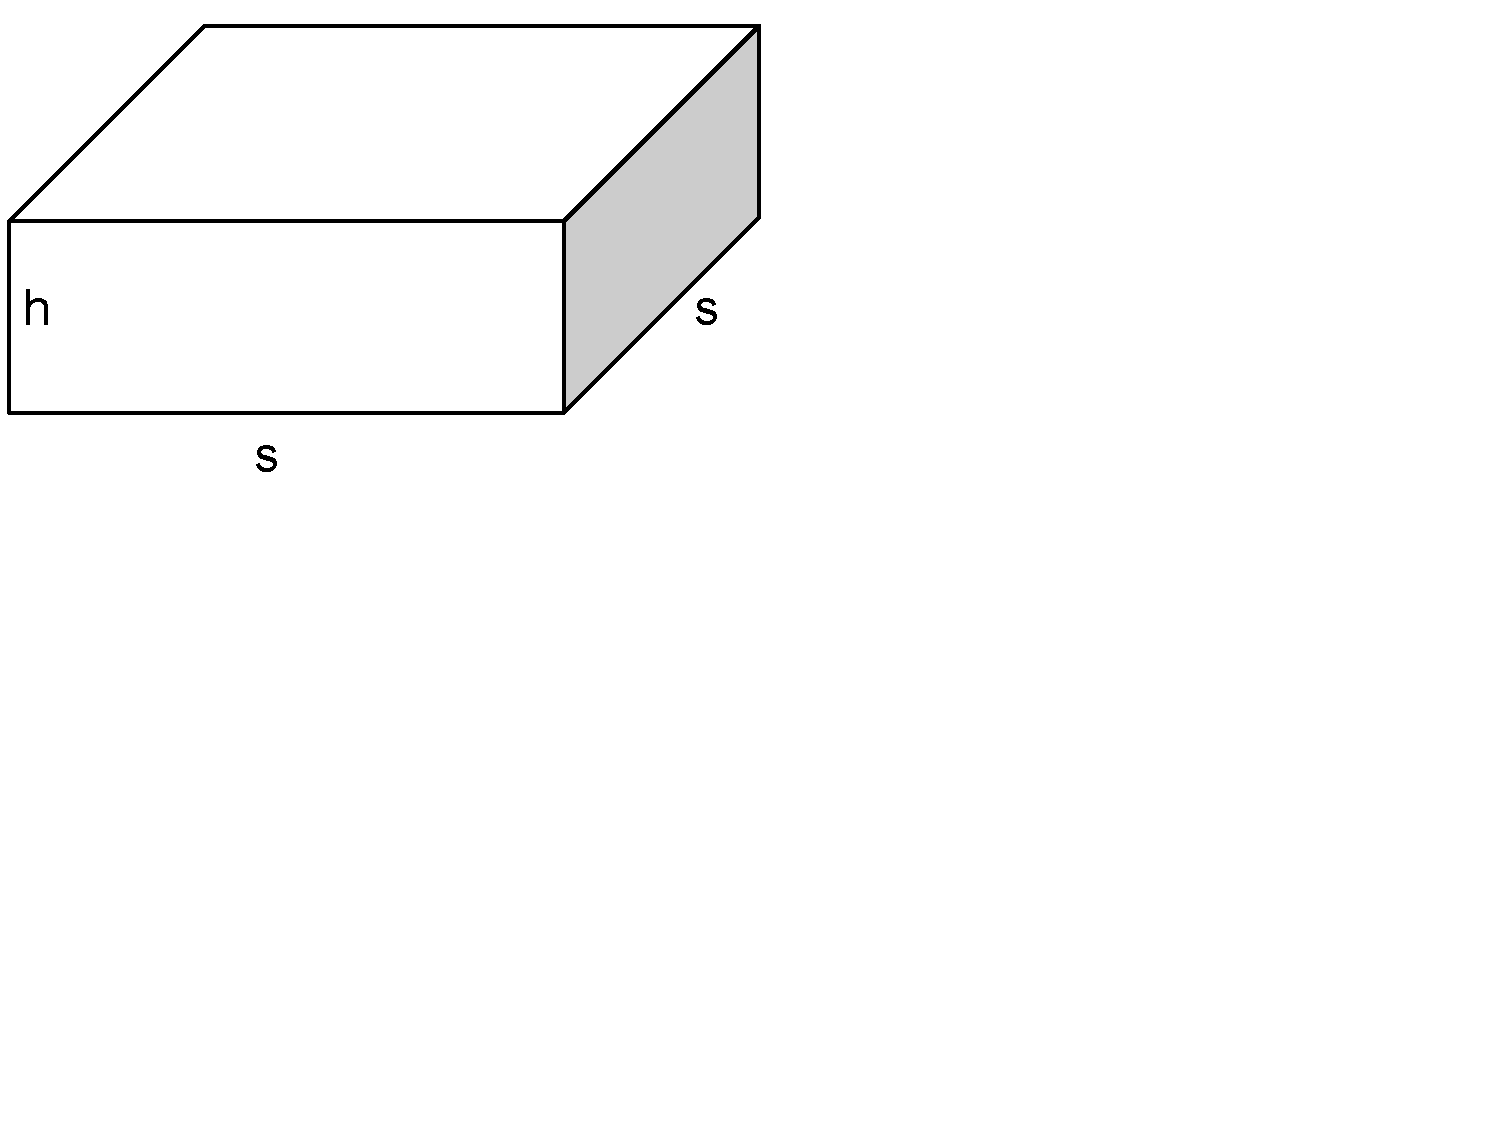
\includegraphics[width=3in]{images/ps03p02.pdf}  
      \end{center} 
      To get the volume, we multiply $\text{length} \times
      \text{width} \times \text{height} = \boxed{s^2 h}$. 
    \end{solution} 

  \item

    \begin{grading}
      2 points. If their answer is wrong but it looks like they're
      trying to calculate the area of each side and add these up, they
      get 1 point. 
    \end{grading}

    \begin{problem}[\vfill]
      Express the surface area of the box in terms of $s$ and $h$.
    \end{problem}

    \begin{solution}

      \textbf{Goal:} Find the surface area of the box in terms of $s$ and $h$. 

      The box has 6 sides. The top and bottom each have area $s^2$, 
      while the other 4 sides each have area $sh$. So, the total
      surface area is $\boxed{2s^2+4sh}$. 
    \end{solution} 

  \item

    \begin{grading}
      3 points. 1 for stating the goal, 1 for using the volume to express $h$ in terms of $s$, 1 for plugging this into the surface area formula.
    \end{grading}

    \begin{problem}[\nstretch{2}]
      If the volume of the box is 120 cubic inches, express the
      surface area of the box as a function of $s$.
    \end{problem}

    \begin{solution}

      \textbf{Goal:} Find surface area in terms of $s$.

      \textbf{Know:}
      \begin{itemize}
      \item surface area = $2s^2 + 4sh$
      \item volume = $s^2 h$ = 120 cubic inches
      \end{itemize}

      We have the surface area in terms of $s$ and $h$, but we want it
      just in terms of $s$. If we can express $h$ in terms of $s$, 
      then we'll be all set.

      Since $s^2 h = 120$, we can solve to find
      $\displaystyle h = \frac{120}{s^2}$. Plugging this into the
      formula for surface area, we get that the surface area will be
      $\displaystyle 2s^2 + 4s \left(\frac{120}{s^2}\right) = \boxed{2s^2 +
        \frac{480}{s}}$.
    \end{solution} 

  \end{enumerate}

\item \label{gottlieb-1.3.30} % 1.3.30

  \begin{workshop}
    Students will need to use the Pythagorean Theorem, but we really want them to figure this out on their own! Rather than telling them to use the Pythagorean Theorem, you might ask them to identify what they want to know (hopefully they will figure out they need the base). How can they use the fact that the rectangle is inscribed in a semicircle? What's special about a semicircle? (It has a radius.) Is there somewhere they can draw that radius that's helpful?
  \end{workshop}

  A rectangle is inscribed in a semicircle of radius $R$, where $R$ is a constant.

  \begin{tikzpicture}[x=0.8in, y=0.8in]
    \draw[fill=lightgray] (-0.6, 0) -- (-0.6, 0.8) -- (0.6, 0.8)
    -- (0.6, 0) -- cycle; %
    \draw[very thick] (-1, 0) -- (1, 0) arc[radius=1, start
    angle=0, end angle=180]; %
  \end{tikzpicture}

  \begin{enumerate}
  \item \label{gottlieb-1.3.30a}

    \begin{grading}
      7.5 points:
      \begin{itemize}[nosep]
      \item 1.5 points for labeling variables and constants in their picture. (In addition to $h$ and $R$, they will most likely need some variable to represent the width or half the width of the rectangle, and they should label this as well.)
      \item 1 for identifying the goal
      \item 1 for writing a formula for area that's consistent with their variables
      \item 1 for recognizing they can use the Pythagorean Theorem to relate variables
      \item 1 for writing a Pythagorean Theorem equation that's consistent with their variables
      \item 1 for solving correctly for the appropriate variable
      \item 1 for plugging back into their area formula
      \end{itemize}
    \end{grading}

    \begin{problem}[\newpage]
      Express the area of the rectangle as a function of the height of the rectangle.

      (Since you're given a picture, you don't need to draw one, but please label the picture above with any variables or constants you use.)
    \end{problem}

    \begin{solution}\

      \textbf{Goal:} Express area in terms of height.

      \textbf{Know:} radius = $R$

      \textbf{Introduce variables:}
      \begin{itemize}[nosep]
      \item $h = $ height of rectangle
      \item $w = $ width of rectangle 
      \end{itemize}

      Here's a picture with our variables:
      \begin{center}
        \begin{tikzpicture}[x=0.8in, y=0.8in]
          \draw[fill=lightgray] (-0.6, 0) -- (-0.6, 0.8) -- (0.6, 0.8) -- (0.6, 0) -- cycle; %
          \draw[very thick] (-1, 0) -- (1, 0) arc[radius=1, start angle=0, end angle=180]; %
          \draw (0.6, 0.4) node[right]{$h$}; %
          \draw[decorate, decoration={brace, mirror}, yshift=-2pt] (-0.6, 0) -- node[yshift=-1em] {$w$} (0.6, 0); %
        \end{tikzpicture}
      \end{center}
      Then, area = $wh$. We want area in terms of just $h$, so we would like to write $w$ in terms of $h$.

      We also know the radius is $R$, and it's most useful to draw this to a corner of the rectangle:
      \begin{center}
        \begin{tikzpicture}[x=0.8in, y=0.8in]
          \draw[fill=lightgray] (-0.6, 0) -- (-0.6, 0.8) -- (0.6, 0.8) -- (0.6, 0) -- cycle; %
          \draw[very thick] (-1, 0) -- (1, 0) arc[radius=1, start angle=0, end angle=180]; %
          \draw (0.6, 0.4) node[right]{$h$}; %
          \draw[decorate, decoration={brace, mirror}, yshift=-2pt] (-0.6, 0) -- node[yshift=-1em] {$w$} (0.6, 0); %
          \draw[blue] (0, 0) -- node[anchor=south east]{$R$} (0.6, 0.8); %
        \end{tikzpicture}
      \end{center}
      Now, we see a right triangle with legs of length $h$ and $\dfrac{w}{2}$ and hypotenuse $R$. So, by the Pythagorean Theorem,
      \begin{align*}
        h^2 + \left( \frac{w}{2} \right)^2 &= R^2 \\
        \left( \frac{w}{2} \right)^2 &= R^2 - h^2 \\
        \frac{w}{2} &= \sqrt{R^2 - h^2} \\
        w &= 2 \sqrt{R^2 - h^2}
      \end{align*}
      We can plug this into our formula for area to get $A = wh = \boxed{ 2h\sqrt{R^2 -h^2}}$.
    \end{solution}

  \item

    \begin{grading}
      4 points:
      \begin{itemize}[nosep]
      \item 1 for identifying the goal
      \item 1 for writing a formula for perimeter that's consistent
        with their variables
      \item 1 for solving their Pythagorean Theorem equation for the
        appropriate variable
      \item 1 for plugging back into their perimeter formula
      \end{itemize}
    \end{grading}

    \begin{problem}[\vfill]
      Express the perimeter of the rectangle as a function of the
      \emph{width} of the rectangle. 
    \end{problem}

    \begin{solution}\

      \textbf{Goal:} Express perimeter in terms of width.

      \textbf{Know:} radius = $R$

      \textbf{Introduce variables:}
      \begin{itemize}[nosep]
      \item $h = $ height of rectangle
      \item $w = $ width of rectangle 
      \end{itemize}

      Here's a picture with our variables:
      \begin{center}
        \begin{tikzpicture}[x=0.8in, y=0.8in]
          \draw[fill=lightgray] (-0.6, 0) -- (-0.6, 0.8) -- (0.6, 0.8) -- (0.6, 0) -- cycle; %
          \draw[very thick] (-1, 0) -- (1, 0) arc[radius=1, start angle=0, end angle=180]; %
          \draw (0.6, 0.4) node[right]{$h$}; %
          \draw[decorate, decoration={brace, mirror}, yshift=-2pt] (-0.6, 0) -- node[yshift=-1em] {$w$} (0.6, 0); %
        \end{tikzpicture}
      \end{center}
      Then, perimeter = $2w+2h$. We want perimeter in terms of just $w$, so we would like to write $h$ in terms of $w$.

      As before, we draw the radius to a corner of the rectangle:
      \begin{center}
        \begin{tikzpicture}[x=0.8in, y=0.8in]
          \draw[fill=lightgray] (-0.6, 0) -- (-0.6, 0.8) -- (0.6, 0.8) -- (0.6, 0) -- cycle; %
          \draw[very thick] (-1, 0) -- (1, 0) arc[radius=1, start angle=0, end angle=180]; %
          \draw (0.6, 0.4) node[right]{$h$}; %
          \draw[decorate, decoration={brace, mirror}, yshift=-2pt] (-0.6, 0) -- node[yshift=-1em] {$w$} (0.6, 0); %
          \draw[blue] (0, 0) -- node[anchor=south east]{$R$} (0.6, 0.8); %
        \end{tikzpicture}
      \end{center}
      Now, we see a right triangle with legs of length $h$ and $\dfrac{w}{2}$ and hypotenuse $R$. So, by the Pythagorean Theorem,
      \begin{align*}
        h^2 + \left( \frac{w}{2} \right)^2 &= R^2 \\
        h^2 &= R^2 - \left( \frac{w}{2} \right)^2  \\
        h &= \sqrt{R^2 - \frac{w^2}{4}}
      \end{align*}
      We can plug this into our formula for perimeter to get $P = 2w+2h = \boxed{2w + 2 \sqrt{R^2 - \frac{w^2}{4}}}$.
    \end{solution}

  \end{enumerate}

\item \label{resources}

  \begin{grading}
    2 points: full credit for any thoughtful response
  \end{grading}

  \begin{problem}[\stretch{0.4}]
    Previously, we asked you to visit the MQC or office hours, or to get together with at least one other student outside of class. Which did you do? If a friend asked you about doing the same thing, what would you recommend they do to get the most out of it?
  \end{problem}

\end{enumerate}
\psreflection{}
\end{document}
